\documentclass[11pt,a4paper]{article}

\usepackage[left=2cm,text={17cm, 24cm},top=3cm]{geometry}
\usepackage[czech]{babel}
\usepackage[utf8]{inputenc}
\usepackage{times}
\usepackage[T1]{fontenc}

\usepackage[ruled,czech,linesnumbered,longend,noline]{algorithm2e}

\usepackage{graphics}
\usepackage{picture}
\usepackage{multirow}

\usepackage{pdflscape}

\newcommand{\myuv}[1]{\quotedblbase #1\textquotedblleft}

\begin{document}
	
	\begin{titlepage}
		\begin{center}
			\Huge
			\textsc{\Huge Vysoké učení technické v~Brně \\ {\huge Fakulta informačních technologií \\}}
			\vspace{\stretch{0.382}}
			{\LARGE Typografie a publikování --\ 3. projekt} \\ {\Huge Tabulky a obrázky}
			\vspace{\stretch{0.618}}
		\end{center}
		{\Large 27. marec 2016 \hfill
			Róbert Kolcún, xkolcu00}
	\end{titlepage}
	
	
	
	%**************************NEXT PAGE******************************************
	\section{Úvodní strana}
	Název práce umístěte do zlatého řezu a nezapomeňte uvést dnešní datum a vaše jméno a příjmení.
	
	\section{Tabulky}
	Pro sázení tabulek můžeme použít buď prostředí \, \texttt{tabbing} \, nebo prostředí \, \texttt{tabular}.
	
	\subsection{Prostředí \, \texttt{tabbing}}
	Při použití \, \texttt{tabbing} \, vypadá tabulka následovně:
	
	\begin{tabbing}
		
		\textbf{Ovoce} \qquad \qquad \= \textbf{Cena} \quad \= \textbf{Množství} \\
		Jablka \> 25,90 \> 3 kg \\
		Hrušky \> 27,40 \> 2,5 kg \\
		Vodní melouny \> 35,-- \> 1 kus
		
	\end{tabbing}
	
	\noindent
	Toto prostředí se dá také použít pro sázení algoritmů, ovšem vhodnější je použít
	prostředí \, \texttt{algorithm} \, nebo \texttt{algorithm2e} \, (viz sekce \ref{sec:algorithm}).
	
	\subsection{Prostředí \, \texttt{tabular}}
	Další možností, jak vytvořit tabulku, je použít prostředí \, \texttt{tabular}. Tabulky pak
	budou vypadat takto\footnote[1]{Kdyby byl problem s~\, \texttt{cline}, \, zkuste se podívat třeba sem:
	http://www.abclinuxu.cz/tex/poradna/show/325037}:

	\medskip
	
	\begin{table}[h]
		\begin{center}
			\catcode`\-=12
			\begin{tabular}{|l|r|r|}
				\hline
				& \multicolumn{2}{|c|}{\textbf{Cena}} 										\\	\cline{2-3}
				\textbf{Měna}	& \textbf{nákup} 						& \textbf{prodej}	\\	\hline
				EUR 			& 27,34 								& 27,42				\\
				GBP				& 33,09									& 33,21				\\
				USD				& 19,87									& 19,95				\\	\hline
			\end{tabular}
			\caption{Tabulka kurzů k~dnešnímu dni}
			\label{tab:Cena}
		\end{center}
	\end{table}
	
	\begin{table}[h]
		\begin{center}
			\catcode`\-=12
			\hfill
			\begin{tabular}{|c|c|}
				\hline
				$A$			&	$\neg A$	\\	\hline
				\textbf{P}	&	N		\\	\hline
				\textbf{O}	&	O~\\	\hline
				\textbf{X}	&	X		\\	\hline
				\textbf{N}	&	P		\\	\hline
			\end{tabular}
			\hfil
			\begin{tabular}{|c|c|c|c|c|c|}
				\hline
				\multicolumn{2}{|c|}{\multirow{2}{*}{$A \wedge B$}}	& \multicolumn{4}{|c|}{$B$}			\\	\cline{3-6}
				\multicolumn{2}{|c|}{}				& \textbf{P} & \textbf{O} & \textbf{X} & \textbf{N}	\\	\hline
				\multirow{4}{*}{$A$}				& \textbf{P} & P & O~& X & N						\\	\cline{2-6}
													& \textbf{O} & O~& O~& N & N						\\	\cline{2-6}
													& \textbf{X} & X & N & X & N						\\	\cline{2-6}
													& \textbf{N} & N & N & N & N						\\	\hline
			\end{tabular}
			\hfil
			\begin{tabular}{|c|c|c|c|c|c|}
				\hline
				\multicolumn{2}{|c|}{\multirow{2}{*}{$A \vee B$}}	& \multicolumn{4}{|c|}{$B$}			\\	\cline{3-6}
				\multicolumn{2}{|c|}{}				& \textbf{P} & \textbf{O} & \textbf{X} & \textbf{N}	\\	\hline
				\multirow{4}{*}{$A$}				& \textbf{P} & P & P & P & P						\\	\cline{2-6}
													& \textbf{O} & P & O~& P & O~\\	\cline{2-6}
													& \textbf{X} & P & P & X & X						\\	\cline{2-6}
													& \textbf{N} & P & O~& X & N						\\	\hline
			\end{tabular}
			\hfil
			\begin{tabular}{|c|c|c|c|c|c|}
				\hline
				\multicolumn{2}{|c|}{\multirow{2}{*}{$A \rightarrow B$}}	& \multicolumn{4}{|c|}{$B$}	\\	\cline{3-6}
				\multicolumn{2}{|c|}{}				& \textbf{P} & \textbf{O} & \textbf{X} & \textbf{N}	\\	\hline
				\multirow{4}{*}{$A$}				& \textbf{P} & P & O~& X & N						\\	\cline{2-6}
													& \textbf{O} & P & O~& P & O~\\	\cline{2-6}
													& \textbf{X} & P & P & X & X						\\	\cline{2-6}
													& \textbf{N} & P & P & P & P						\\	\hline
			\end{tabular}
			\hfill \hfil
			\caption{Protože Kleeneho trojhodnotová logika už je \myuv{zastaralá}, uvádíme si zde příklad čtyřhodnotové logiky}
			\label{tab:Kleen}
		\end{center}
	\end{table}



	\pagebreak
	%**************************NEXT PAGE******************************************

	\section{Algoritmy}
	\label{sec:algorithm}
	Pokud budeme chtít vysázet algoritmus, můžeme použít prostředí \texttt{algorithm}\footnote[2]{\raggedright Pro nápovědu, jak zacházet s~prostředím \, \texttt{algorithm}, můžeme zkusit tuhle stránku:
		http://ftp.cstug.cz/pub/tex/CTAN/macros/latex/contrib/algorithms/algorithms.pdf.} nebo \texttt{algorithm2e}\footnote[3]{Pro \, \texttt{algorithm2e} zase tuhle:
		http://ftp.cstug.cz/pub/tex/CTAN/macros/latex/contrib/algorithm2e/algorithm2e.pdf.}. \linebreak
	Příklad použití prostředí \, \texttt{algorithm2e} \, viz Algoritmus \ref{alg:FastSlam}.
	
	\bigskip
	\bigskip
	
	\begin{algorithm}[H]
		\SetKwInput{Input}{Input}
		\SetKwInOut{Output}{Output}
		
		\SetNlSty{}{}{:}
		\SetInd{1em}{1em}
		\SetNlSkip{-1.33em} %Posunutie cislovanie
		
		\Input{$(X_{t-1},u_t,z_t)$}
		\Output{$X_t$}
		\BlankLine
		\Indp \Indp
		$\overline{X_t} = X_t = 0$\\
		\For{$k=1$ \textnormal{to} $M$}
		{ 
			$x_t^{[k]} =$ \emph{sample\_motion\_model}$(u_t,x_{t-1}^{[k]})$		\\
			$w_t^{[k]} =$ \emph{measurement\_model}$(z_t,x_t^{[k]},m_{t-1})$	\\
			$m_t^{[k]} = updated\_occupancy\_grid(z_t,x_t^{[k]},m_{t-1}^{[k]})$	\\
			$\overline{X_t} = \overline{X_t} + \langle x_x^{[m]},w_t^{[m]}\rangle$
		}
		\For{$k=1$ \textnormal{to} $M$}
		{
			draw $i$ with probability $\approx w_t^{[i]}$\\
			add $\langle x_x^{[k]},m_t^{[k]}\rangle$ to $X_t$\\
		}
		\Return{$X_t$}
		
		\caption{\textsc{Fast}SLAM}
		\label{alg:FastSlam}
	\end{algorithm}
	
	\medskip
	
	\section{Obrázky}
	Do našich článků můžeme samozřejmě vkládat obrázky. Pokud je obrázkem fotografie,
	můžeme klidně použít bitmapový soubor. Pokud by to ale mělo být nějaké schéma nebo
	něco podobného, je dobrým zvykem takovýto obrázek vytvořit vektorově.
	
	\begin{figure}[h]
		\begin{center}
		\scalebox{0.4}
		{
			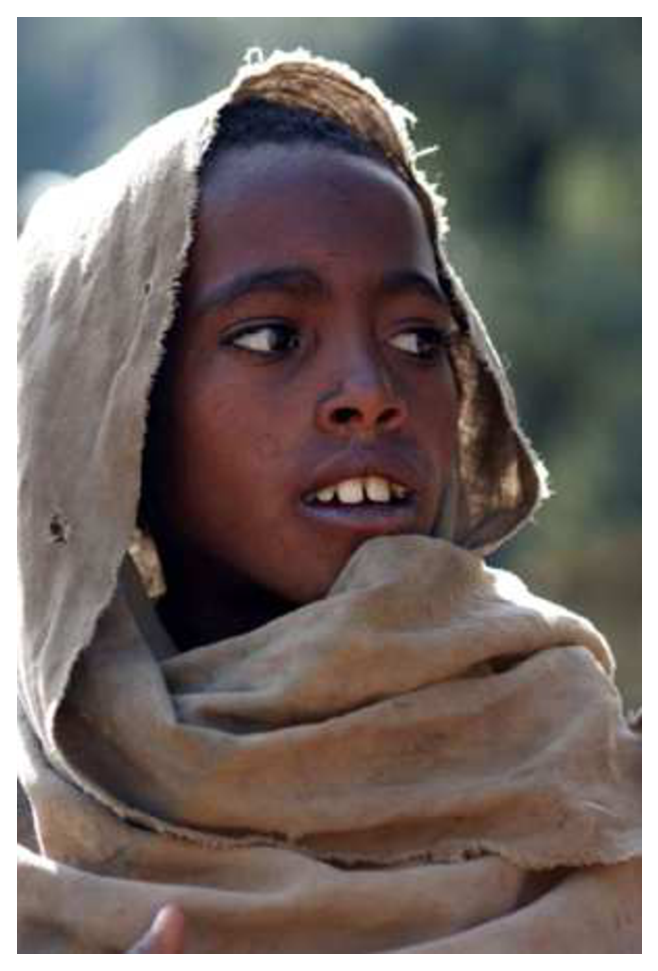
\includegraphics{etiopan}
			\reflectbox{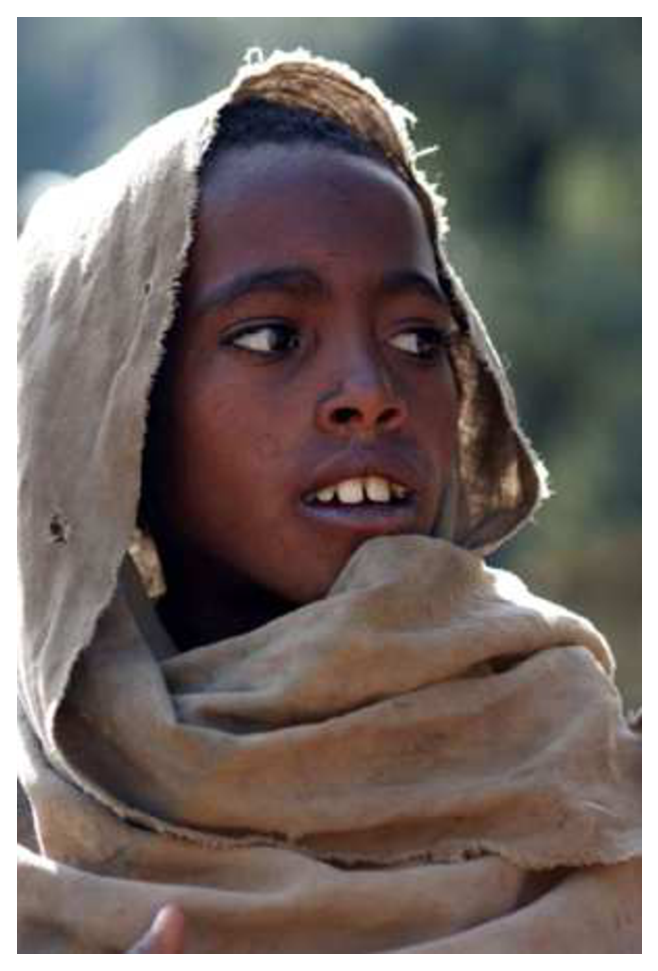
\includegraphics{etiopan}}
		}
		\caption{Malý Etiopánek a jeho bratříček}
		\label{pic:Etiopie}
		\end{center}
	\end{figure}
	
	
	
	
	\pagebreak
	%**************************NEXT PAGE******************************************
	Rozdíl mezi vektorovým \ldots
	
	\begin{figure}[h]
		\begin{center}
			\scalebox{0.4}{
\includegraphics{oniisan}}
			\caption{Vektorový obrázek}
			\label{pic:Vektor}
		\end{center}
	\end{figure}
	
	\ldots \, a bitmapovým obrázkem
	
	\begin{figure}[h]
		\begin{center}
			\scalebox{0.6}{
\includegraphics{oniisan2}}
			\caption{Bitmapový obrázek}
			\label{pic:Bitmap}
		\end{center}
	\end{figure}
	
	\noindent
	se projeví například při zvětšení
	
	Odkazy (nejen ty) na obrázky \ref{pic:Etiopie}, \ref{pic:Vektor} a \ref{pic:Bitmap}, na  
	tabulky \ref{tab:Cena} a \ref{tab:Kleen} a také na algoritmus \ref{alg:FastSlam} jsou udělány pomocí 
	křížových odkazů. Pak je ovšem potřeba zdrojový soubor přeložit dvakrát.
	
	Vektorové obrázky lze vytvořit i přímo v~\LaTeX, například pomocí prostředí \, \texttt{picture}.
	
	
	\pagebreak
	%**************************NEXT PAGE******************************************
	\begin{landscape}
		\begin{figure}[h]
			\begin{picture}(570,330)(-60,0)
			\linethickness{1pt}
			
			\put(475,240){\circle{70}}
			
			\put(0,0){\framebox(570,300)}	%FrameBox pre cely obrazok
			\put(75,40){\line(0,1){115}}
			\put(75,155){\line(1,0){120}}
			
			\put(195,140){\framebox(160,30)}
			\put(135,119){\framebox(380,20)}
			\put(356,140){\framebox(140,8)}
			\put(135,118){\line(1,-1){38}}
			
			\put(110,40){\line(0,1){40}}
			\put(110,80){\line(1,0){100}}
			\put(210,80){\line(3,-1){120}}
			
			\put(220,77){\line(0,1){33}}
			\put(220,110){\line(1,0){290}}
			\put(510,110){\line(0,-1){45}}
			
			\put(255,65){\line(1,0){260}}
			\put(515,40){\line(0,1){25}}
			
			\linethickness{6pt}
			\put(10,40){\line(1,0){550}}
			\end{picture}
			\caption{Vektorový obrázok v~prostředí \texttt{picture}}
		\end{figure}
	\end{landscape}
	
	
	
	
\end{document}